{\fontsize{35pt}{50pt} \textbf{Explain any rule-based model using game theory}\par}

\vspace{10mm}

\begin{figure}[h]
\begin{center}

\includegraphics[scale=0.223]{./../img/make-things-clearer.png}
\caption{Making things clearer}
\end{center}
\end{figure}

With the rise of digitalisation, one of the key challenges of any company is to understand well enough the impact of the algorithms that it uses. Although we hear a lot about highly sophisticated algorithms such as neural networks, often times in big industries algorithms based on simple rules are more used than fancy machine learning approaches. Note: in this article we will call "model" a group of algorithms. \textit{Explainability} is the concept that a model can be explained in a way that “makes sense” to a human being at an acceptable level (definition from \href{https://c3.ai/glossary/machine-learning/explainability/}{c3.ai}). \\

Let's say an online shop wants to target certain clients. More specifically, we'll imagine the company wants to focus on the oldest and wealthiest European clients. Thus, the management decides to select clients satisfying the following criteria: 

- older than 40 years old \\
- based in Europe \\
- income higher than 100K \\

\begin{center}
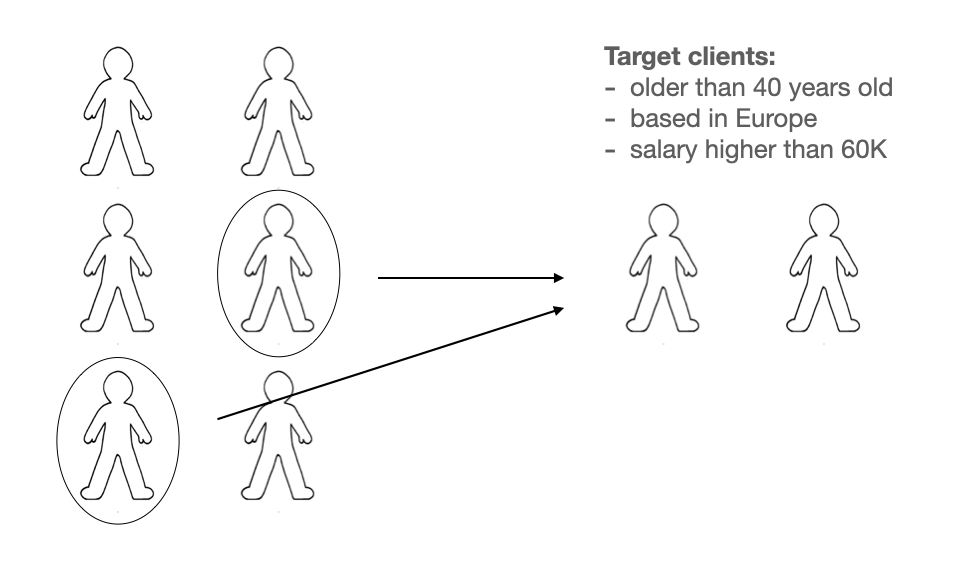
\includegraphics[scale=0.5]{./../img/clients-filter.png}
\end{center}

We call those criteria "rules".

Since there are just a few rules involved here, there is no real need for explainability. But let's say now the management decides to fine-tune the selection and starts to add more rules:

- older than 40 years old \\
- based in Europe \\
- income higher than 100K \\
- lives in a house \\
- client since at least 3 years \\
- purchased no more than 10 products \\
- has a least 2 children \\
- bought one swimming suit \\
- had a dog in the past \\
- ...

As you can imagine, the possibilities are endless. When using such rules, we may want to know: \textbf{what rules are important here? Which one is really contributing to the selection of clients? Can we rank these rules by importance?} This is exactly what model explainability tries to find out. In other words, it aims at finding what variables are responsible for the result we have. We will present a method that helps answering the question. \\

Let us use our first illustrative example and assume our client data are composed of age, location and income. The below picture is a summary of our (simplified) database. 

\begin{center}
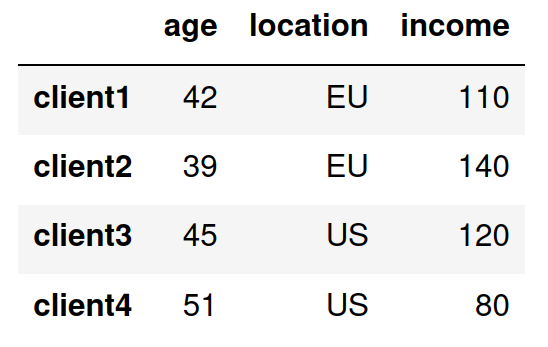
\includegraphics[scale=0.3]{./../img/data-simple-example.png}
\end{center}

The used rules are the following:

- rule 1: age>40 \\
- rule 2: location="EU" \\
- rule 3: income>100 \\

Now we want to know what rule is really important here? Which one is the most "selective"? One intuitive way to answer this question is to remove each rule one by one, and see how it changes the results. \\

We note that when using the three rules, we end up with 25\% of clients since only one client is not filtered out. 

\begin{center}
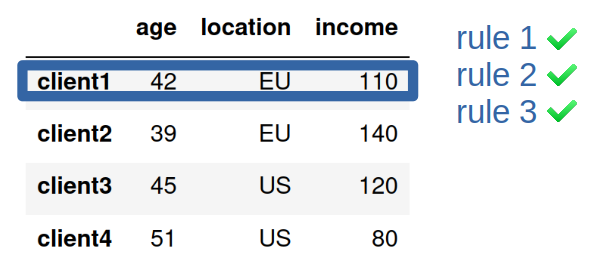
\includegraphics[scale=0.3]{./../img/3rules.png}
\end{center}


When removing only rule 1 (age) we end up with 50\% of the clients. 

When removing only rule 2 (location) we end up with 50\% of the clients.

Thus, our first analysis suggests that rule 1 and rule 2 are equally important. \\

But is this analysis complete? No. \\

To compare the impact of rule 1  and rule 2 we can't just remove these rules one by one since rule 3 and rule 2 both filter out client4. Thus, removing rule 1 or rule 2 doesn't make any difference on the final result (50\% in both cases). Because of this overlapping  effect, we need to look at other combinations. For example, what happen if we use \textit{only} rule 1 or rule 2? With rule 1 only, only one client is filtered out. With rule 2 only, two clients are filtered out. \textbf{Unlike our previous conclusion, here rule 2 seems more selective (and thus more important) than rule 1}. \\

\begin{figure}[h]
\begin{center}
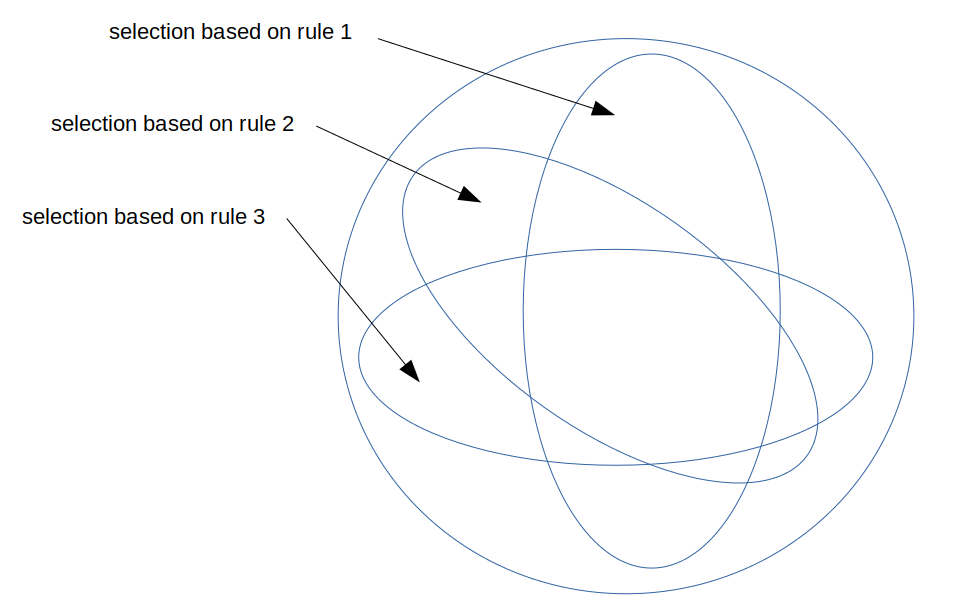
\includegraphics[scale=0.3]{./../img/overlaps.png}
\caption{Overlapping rules}
\end{center}
\end{figure}

To sum up, assessing the rule importance requires us to go over all possible combinations. \\

Now here comes the link with game theory. 
Game theory is a field that consists in analyzing the interactions of individuals (also called \textit{agents}) within a society. We typically look at what contribution an agent brings to the society. How does it link to our problem? Instead of having individuals as agents, let's say the rules are the agents. We want to see what contribution each rule brings to the model. \\

Since a rule can be added or removed, the total possible combinations of rules is $2^R$ with $R$ the number of rules in total. We can draw the different combinations in a powerset (R1, R2, R3 are the respective rules):

\begin{center}
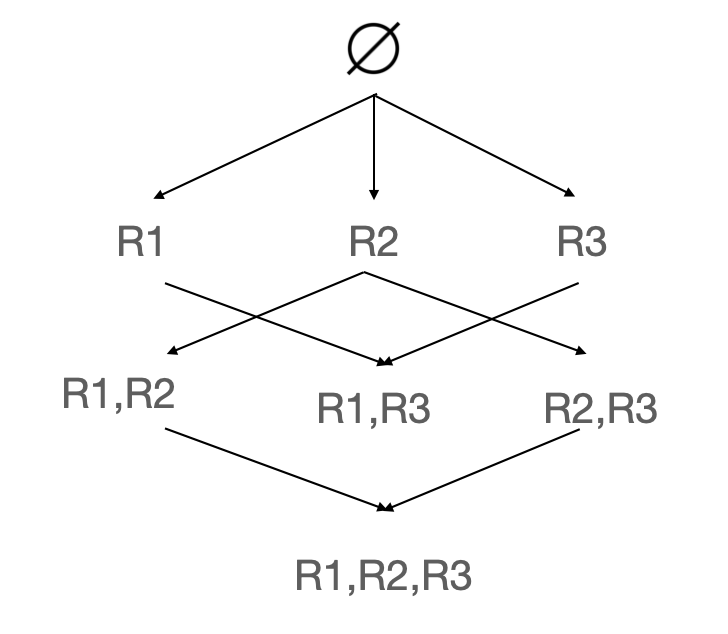
\includegraphics[scale=0.6]{./../img/powerset.png}
\end{center}

We can see here that the number of combinations is $2^3 = 8$. \\

We now want to compute the contribution of each rule. The method proposed below is largely inspired by the article \href{https://arxiv.org/pdf/1705.07874.pdf}{"A Unified Approach to Interpreting Model Predictions"}. The authors show that a way to assess variable importance is to test all combinations and see how each one impact the result. In our use case, the variables (called "feature" in the article) are the \textbf{rules} themselves. The main assumption behind this approach is that the items explaining the model follow a linear relationship:

$$g(z) = \phi_0 + \sum_{i=1}^M \phi_i z_i$$

Let's dive a bit more in the parameters. \\

$g$ is the \textit{explanation} model. It's simply the total effect of the rules on the result.

$z \in \{0,1\}^M$ are all possible combinations of rules. $0$ indicates that the rule is removed from the model, $1$ indicates that a rule is added to the model. As an illustration, $(0,1,0)$ is when only rule 2 is used.

$M$ is the number of rules. 

$\phi_i \in \mathbb{R}$ are the Shapley values. The Shapley values reflect the importance of a rule in the model. As an example, if Shapley(rule 1) = 3 and Shapley(rule 2) = 5 it shows that rule 2 contributes more to the model than rule 1. The rationale behind such values are based on some principles that we won't elaborate here but that are well described in the article. \\

\begin{center}
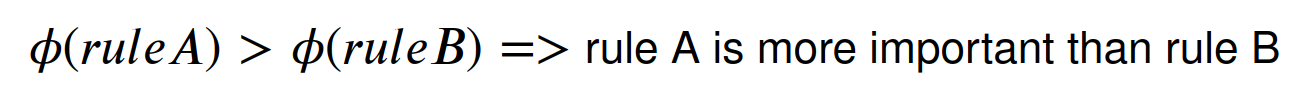
\includegraphics[scale=0.2]{./../img/rule-shapley.png}
\end{center}

The equation above shows us that the Shapley values can be found using an \href{https://en.wikipedia.org/wiki/Ordinary_least_squares}{OLS} method.

$$\phi = (z^Tz)^{-1}z^Ty$$

In our example:

$$z = \begin{pmatrix}
0 & 0 & 0 & 1\\
1 & 0 & 0 & 1\\
0 & 1 & 0 & 1\\
0 & 0 & 1 & 1\\
1 & 1 & 0 & 1\\
1 & 0 & 1 & 1\\
0 & 1 & 1 & 1\\
1 & 1 & 1 & 1
\end{pmatrix}$$

Note: the last column stands for the intercept. It's common practice to use the intercept when the variables are not centered, which is the case here.

$$y = g(z) = \begin{pmatrix}
1 \\
0.75 \\
0.5 \\
0.75 \\
0.25 \\
0.5 \\
0.5 \\
0.25
\end{pmatrix}$$

$y$ is the proportion of selected clients for each rule combination. \\

Now a small subtlety. So far, all combinations are weighted the same. But the authors propose to penalize mixed combinations (e.g. [0,0,1,1]) and encourage more "pure" combinations (e.g. [0,1,1,1]). The intuition behind such behaviour is well explained on \href{https://christophm.github.io/interpretable-ml-book/shapley.html}{Christoph Molnar’s website}: \\

"We learn most about individual features if we can study their effects in isolation. If a coalition [ndlr combination] consists of a single feature, we can learn about this feature’s isolated main effect on the prediction. If a coalition consists of all but one feature, we can learn about this feature’s total effect (main effect plus feature interactions). If a coalition consists of half the features, we learn little about an individual feature’s contribution, as there are many possible coalitions with half of the features."

The weights are thus defined as such:

$$\omega_{z_i} = \frac{R-1}{C_{|z_i|}^R |z_i|(R-|z_i|)}$$

with $|.|$ being the number of non-zero elements in $z_i$. The proof of this formula can be found in the \href{https://proceedings.neurips.cc/paper/2017/hash/8a20a8621978632d76c43dfd28b67767-Abstract.html}{supplementary material} of the article. \\

Note that in our simple example with 3 rules only, the weights are all the same. \\

The implementation of the Shapley values can be found on the \href{https://shap.readthedocs.io/en/latest/example_notebooks/tabular_examples/model_agnostic/Simple%20Kernel%20SHAP.html}{Shap's documentation} and won't be detailed here. The critical part in our use case is to properly define the "prediction" function. For a specific combination of rules, this function returns $0$ if the client is filtered out, 1 otherwise. In other words, if all rules are true, the probability for a client to be selected is 1. \\

We first store the rules we want to assess in a dictionary. The Python function \textit{eval} will be very convenient to test whether a condition is satisfied.

\lstset{language=Python}
\lstset{frame=lines}
\lstset{caption={prediction function}}
\lstset{label={lst:code_direct}}
\lstset{basicstyle=\footnotesize}
\begin{lstlisting}

dict_rules = {
    'rule1':'age>40',
    'rule2':'location=="EU"',
    'rule3':'income>100'
}

def prediction(client_row, activated_rules):
    rules_res = []
    if activated_rules[0]==1:
        age = client_row['age']
        rules_res.append(eval(dict_rules['rule1']))
    if activated_rules[1]==1:
        location = client_row['location']
        rules_res.append(eval(dict_rules['rule2']))
    if activated_rules[2]==1:
        income = client_row['income']
        rules_res.append(eval(dict_rules['rule3']))
    if False not in rules_res:
        return 1
    return 0

\end{lstlisting}

The code of the example can be found on my \href{https://github.com/savoga/shap-explain}{dedicated repo}. \\

The Shapley value computation shows that rule 2 is the most important one. Then comes rule 1 and finally rule 3. We note that all rules contribute negatively to our results. This is expected since adding a rule necessarily filter out more clients. Based on these results, the management can decide for example to remove rule 3 since it's not contributing much to the client selection. Alternatively, it can also decide to remove rule 2 that may be too selective.

\begin{center}
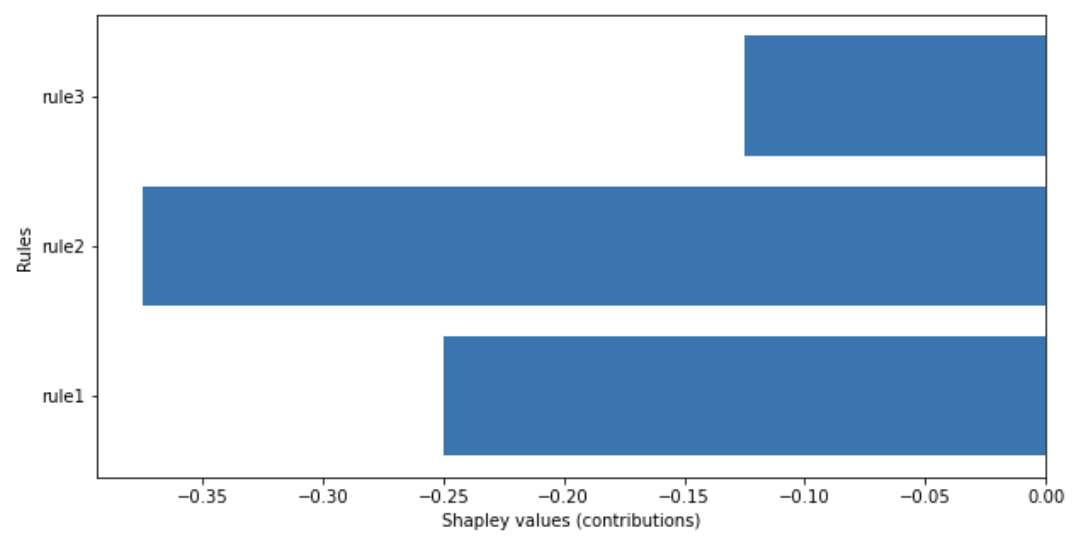
\includegraphics[scale=0.6]{./../img/shapley-results.png}
\end{center}

In this article I have presented a method to assess the importance of rules that compose any model. I first introduced an intuitive method that is unfortunately incomplete. Then I showed a method based on game theory that consider all possible cases to correctly assess the model. I finally gave some references to go deeper in the understanding of the theory. I hope some materials can be reused for your use case. Have fun!


\vspace{10mm}